\lstinputlisting[language=bash,basicstyle=\small]{python_codes/fieldstone_112/keywords}

\begin{center}
\inpython~Code at \url{https://github.com/cedrict/fieldstone/tree/master/python_codes/fieldstone_112}
\end{center}

\par\noindent\rule{\textwidth}{0.4pt}

%%%%%%%%%%%%%%%%%%%%%%%%%%%%%%%%%%%%%%%%%%%%%%%%%%%%%%%%%%%%%%%%%%%%%%%%%%%%%%%%%%%%%%%%%%%%%%%%%%%%


This \stone showcases the MINI (Section~\ref{pair:mini}), 
$P_2\times P_1$ (Section~\ref{ss:p2p1}), $Q_2\times Q_1$ (Section~\ref{ss:pairq2q1}) 
and Crouzeix-Raviart  (Section~\ref{sec:crouzeix-raviart})
elements which are used to solve the manufactured solution problem "Donea \& Huerta" (see Section~\ref{mms1}).

The mesh is composed of $nel_x \times nel_y$ elements which are cut in half via the same diagonal (NW-SE) into 2 triangles
for simplicity: 

\begin{center}

\includegraphics[width=7cm]{python_codes/fieldstone_112/results/grid_quads}
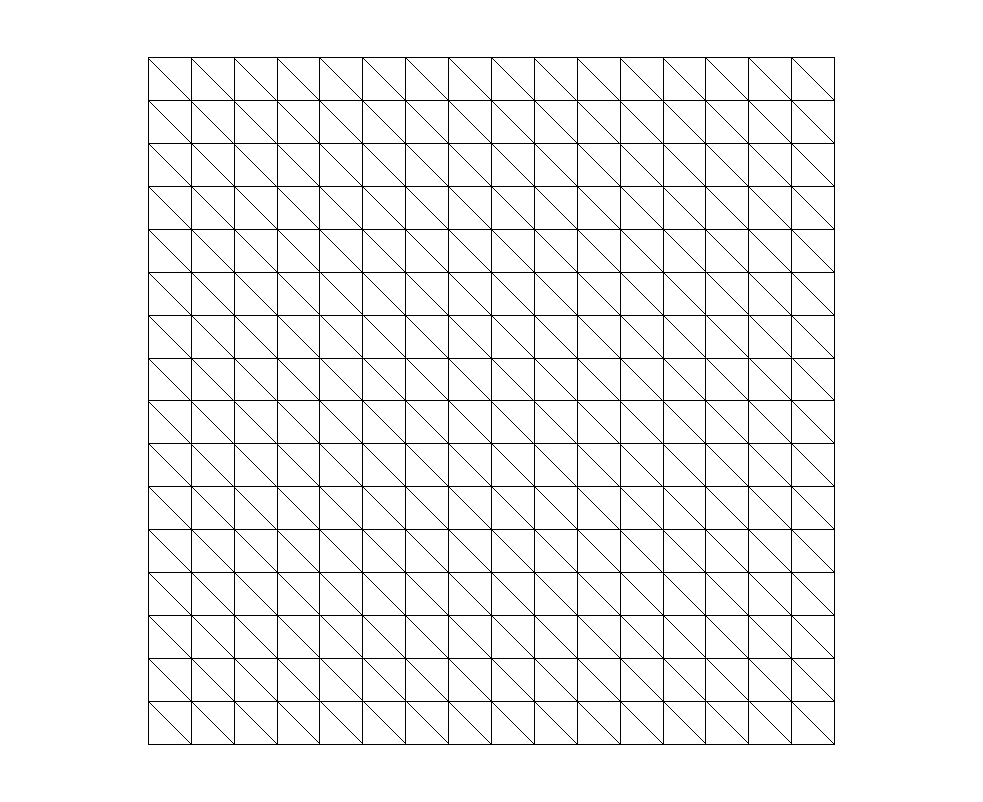
\includegraphics[width=7cm]{python_codes/fieldstone_112/results/grid_triangles}\\
{\captionfont Quadrilaterals and triangles mesh for a resolution of $16\times 16$ cells.} 
\end{center}

A pressure dof is fixed so remove the nullspace and the obtained pressure field
is then normalised so that $\int_\Omega p dV = 0$.

\begin{center}
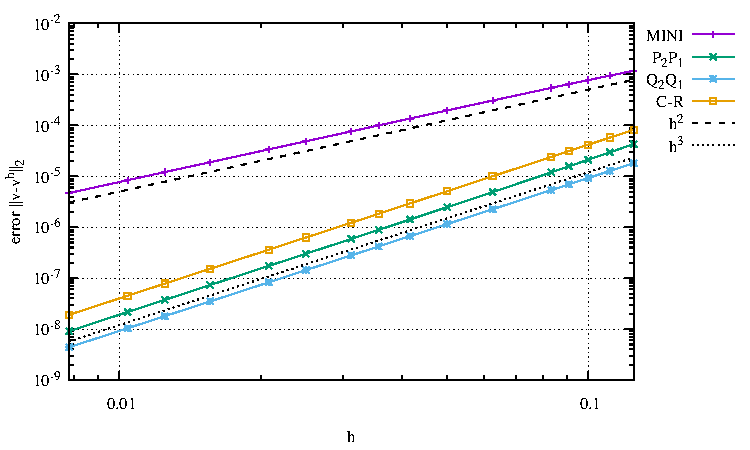
\includegraphics[width=8cm]{python_codes/fieldstone_112/results/errors_V.pdf}
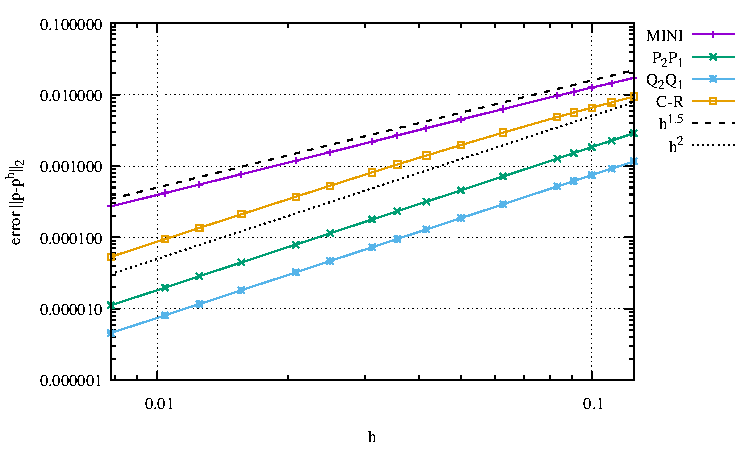
\includegraphics[width=8cm]{python_codes/fieldstone_112/results/errors_P.pdf}\\
{\captionfont Velocity (left) and pressure (right) $L_2$ error as a function of the element size $h$}
\end{center}

\begin{center}
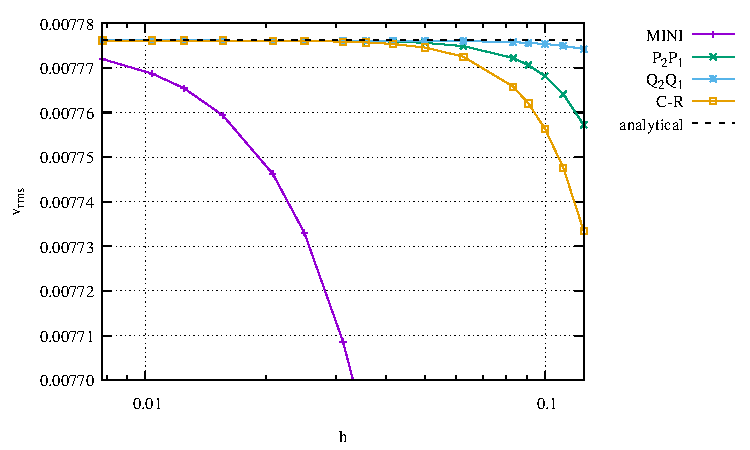
\includegraphics[width=9cm]{python_codes/fieldstone_112/results/vrms.pdf}\\
{\captionfont Root mean square velocity as a function of of the element size $h$}
\end{center}

\begin{center}
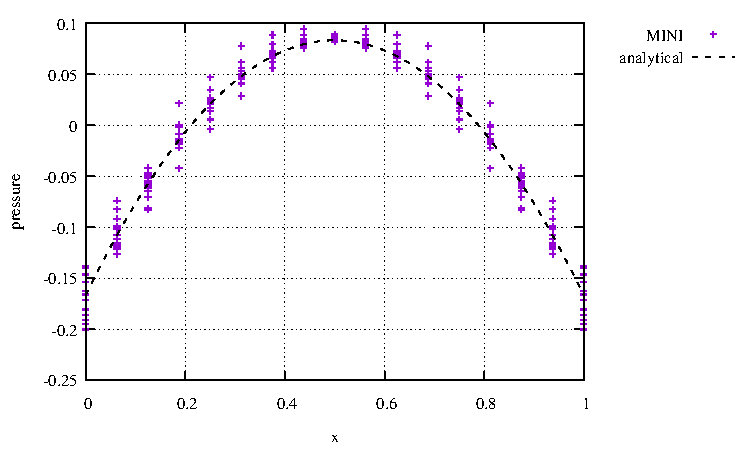
\includegraphics[width=8cm]{python_codes/fieldstone_112/results/pressMINI}
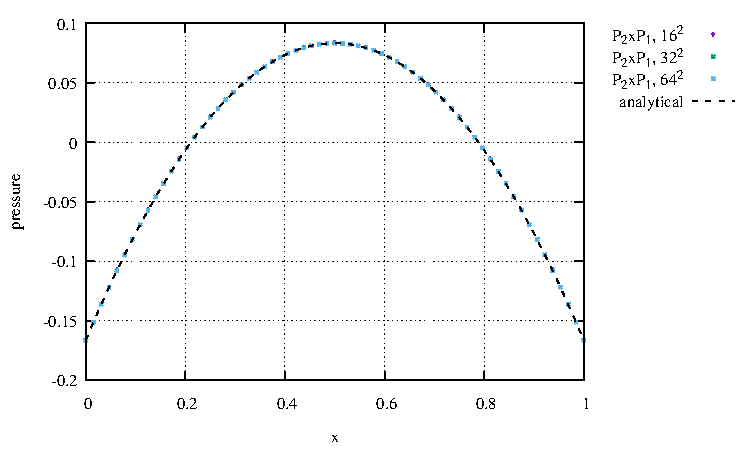
\includegraphics[width=8cm]{python_codes/fieldstone_112/results/pressP2P1}\\
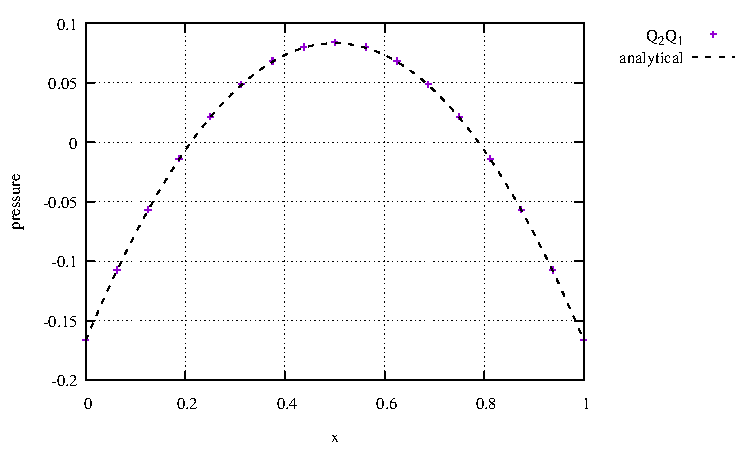
\includegraphics[width=8cm]{python_codes/fieldstone_112/results/pressQ2Q1}
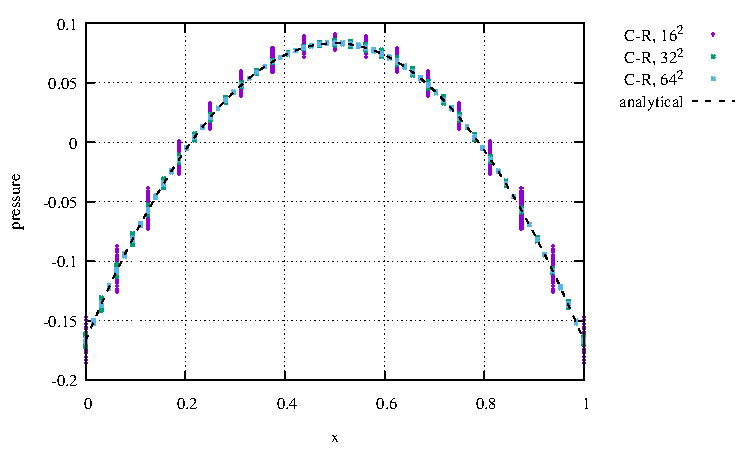
\includegraphics[width=8cm]{python_codes/fieldstone_112/results/pressCR}\\
{\captionfont Pressure field as a function of the $x$-coordinate on a $16\times16$,
$32\times 32$ and $64\times 64$ mesh.} 
\end{center}

TODO: implement Q2Pm1, SolCx, SolVi, SolKz, cylindrical sinker + mesh.
compare accuracy wrt ndofs

check and probably remove stone 46, 47 ?
